%%%%%%%%%%%%%%%%%%%%%%%%%%%%%%%%%%%%%%%%%%%%%%%%%%%%%%%%%%%%%%%%%%%%%%
%     File: ExtendedAbstract_imple.tex                               %
%     Tex Master: ExtendedAbstract.tex                               %
%%%%%%%%%%%%%%%%%%%%%%%%%%%%%%%%%%%%%%%%%%%%%%%%%%%%%%%%%%%%%%%%%%%%%%

\section{Aerial-D Dataset Construction}
\label{sec:approach}

\subsection{Source Datasets}

The AerialD dataset is constructed from two primary sources of aerial imagery with fundamentally different annotation paradigms. The iSAID dataset provides instance segmentation annotations with 655,451 instances across 15 object categories including ships, vehicles, planes, buildings, and infrastructure elements such as harbors and bridges. The dataset contains 2,806 high-resolution aerial images with varying dimensions and spatial resolutions ranging from 0.1m to 4.5m per pixel. In contrast, the LoveDA dataset offers semantic segmentation annotations capturing land cover patterns across 5,987 images at 1024×1024 resolution with 0.3m spatial resolution. It provides pixel-level classification into six categories: buildings, roads, water bodies, agricultural areas, forests, and barren land.

These complementary datasets ensure comprehensive coverage of both discrete objects and continuous landscape features commonly encountered in aerial imagery analysis. The combination enables our pipeline to generate referring expressions for individual object instances from iSAID while also supporting semantic region descriptions from LoveDA's land cover classifications.

\subsection{Rule-Based Expression Generation}

In order to generate referring expressions for the aerial imagery datasets, we take the instance segmentation datasets and semantic segmentation datasets (iSAID and LoveDA) and transform their annotated objects into targets for natural language descriptions. Since iSAID contains very high-resolution images up to 13,000 pixels, we first extract 480×480 patches using a sliding window with overlap to capture manageable regions containing valid instances. We take each individual instance from the annotations, group similar instances together using DBSCAN clustering, and also create category-level groups that encompass all instances of the same type, then try to assign referring expressions based on the characteristics we can derive from the existing annotations.

The core challenge is figuring out how to describe these objects using only what we know from their bounding boxes, masks, and categories. We utilize the bounding box coordinates to understand where each object sits within the image patch. As shown in Figure \ref{fig:rule_example}, we divide each patch into a three-by-three grid marked with dotted lines, so we can say an object is "in the top right" or "in the center". When we have multiple objects of the same type, we also check if any are in extreme positions like the topmost or leftmost instance of that category.

Since we also have the pixel masks for each object, we can analyze their colors by looking at HSV values to distinguish between light and dark objects, and various chromatic colors. However, we avoid using color descriptions for buildings and water since these typically show mixed colors that aren't useful for identification.

We also create relationships between nearby objects by calculating angles between their positions, allowing us to generate expressions like "the ship to the left of the harbor" or "the vehicle above the building". The system uses eight directional relationships: above, below, to the left of, to the right of, and the four diagonal directions.

All these rules combine to generate various referring expressions for each object, as demonstrated in Figure \ref{fig:rule_example} where a single plane generates multiple possible descriptions including "the plane in the top right", "the light plane in the top right", and versions with relational descriptions. However, the biggest challenge emerges when multiple objects end up with identical characteristics and generate the exact same expressions, creating ambiguous references where one phrase could describe multiple different objects. We solve this fundamental problem by taking the set of all expressions for all objects and targets in each image, matching them against each other to find duplicates, and when we find expressions that are identical, we cancel both expressions out and discard them as ambiguous. This ensures every remaining phrase points to exactly one target.

\begin{figure*}[t]
\centering
\begin{minipage}{0.5\textwidth}
\centering
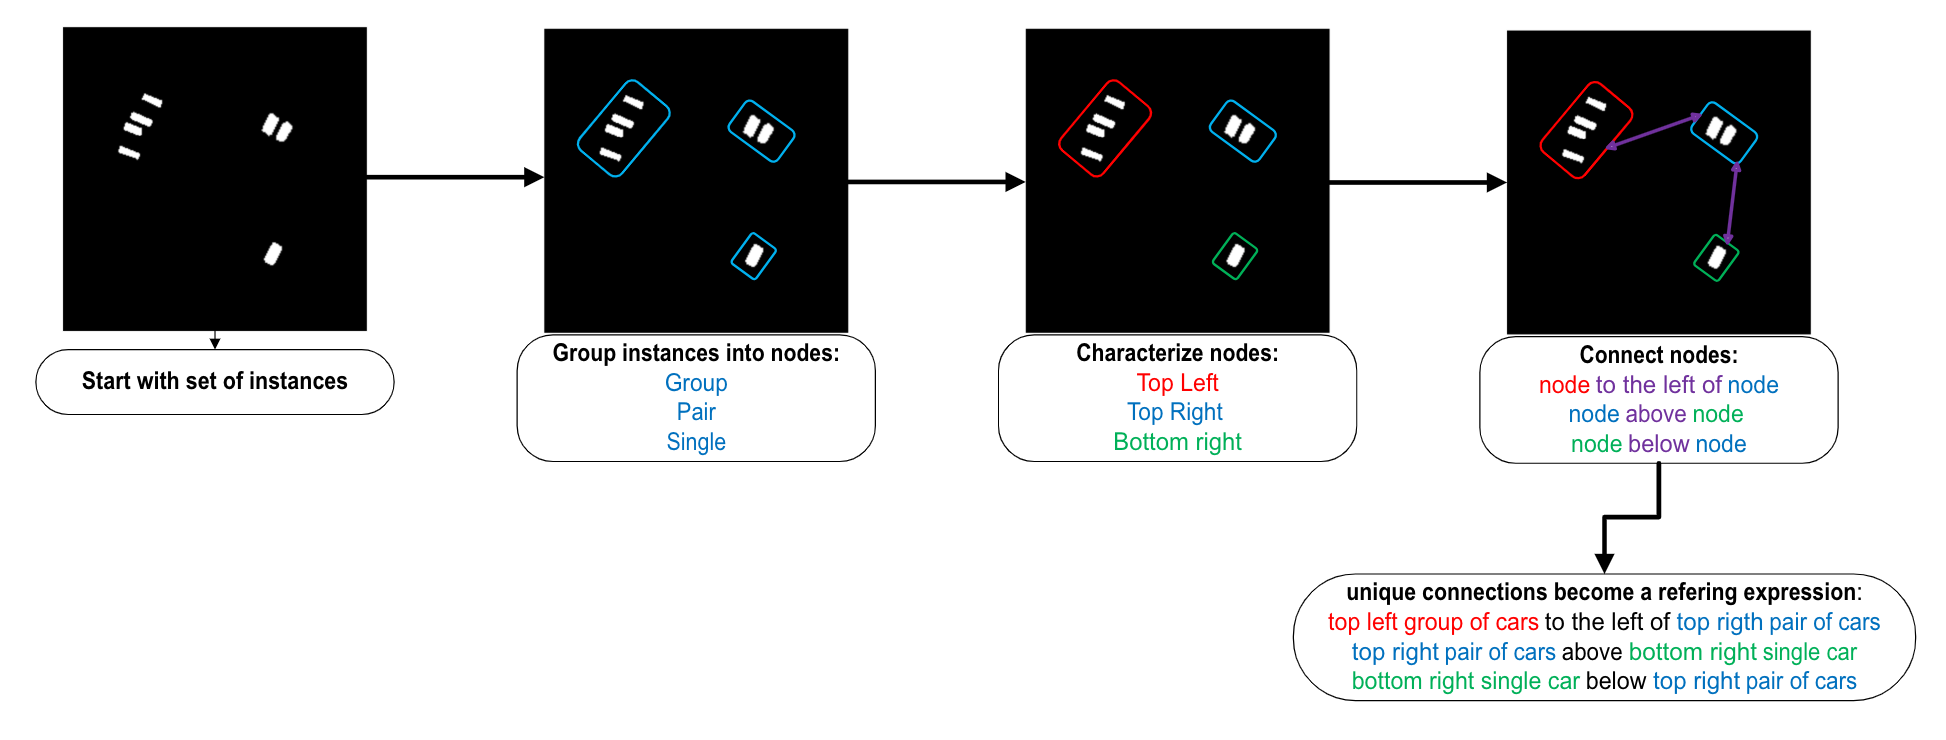
\includegraphics[width=0.7\textwidth]{./images/rule_based_generation.png}
\end{minipage}%
\begin{minipage}{0.5\textwidth}
\centering
\hspace{-1cm}
\raisebox{-0.3\height}{%
\resizebox{\textwidth}{!}{%
\footnotesize
\begin{tabular}{@{}ll@{}}
\toprule
\textbf{Rule Type} & \textbf{Example Instance} \\
\midrule
Category & "plane" \\
Grid Position & "in the top right" \\
Extreme Position & None \\
Color Classification & "light" \\
Directional Relations & "to the bottom right of a plane" \\
& "to the top right of a plane" \\
\midrule
\multicolumn{2}{l}{\textbf{Final Expressions}} \\
\multicolumn{2}{l}{"the plane in the top right"} \\
\multicolumn{2}{l}{"the light plane in the top right"} \\
\multicolumn{2}{l}{"the plane in the top right to the bottom right of a plane"} \\
\multicolumn{2}{l}{"the light plane in the top right to the bottom right of a plane"} \\
\multicolumn{2}{l}{"the plane in the top right to the top right of a plane"} \\
\multicolumn{2}{l}{"the light plane in the top right to the top right of a plane"} \\
\bottomrule
\end{tabular}%
}%
}
\end{minipage}
\caption{Example of rule generation for a single instance. The highlighted plane in the top right section demonstrates how the system assigns spatial, visual, and relational rules that will later be combined into referring expressions.}
\label{fig:rule_example}
\end{figure*}


\subsection{LLM Expression Generation}
While rule-based expression generation provides a solid foundation for referring expression data, these expressions suffer from significant limitations in language variation and visual detail coverage. The rule-based approach produces linguistically constrained expressions with limited wording variations and lacks the ability to reference contextual elements beyond predefined source dataset categories.

To address these limitations, we employ multimodal Large Language Models (LLMs) to enhance our dataset by providing both images and expressions as input, enabling the models to rewrite and improve the original referring expressions. We target enhancement from two complementary angles, as illustrated in Figure \ref{fig:llm_enhancement_example}. The first approach focuses primarily on linguistic variation, emphasizing natural language diversity while minimizing visual attention, thereby generating rich lexical alternatives for each rule-based expression. The second approach grounds improvements in visual analysis, where the model analyzes surrounding contextual features within the image around the target object. To facilitate precise localization, we provide bounding box annotations that direct the model's attention to the specific target region, as demonstrated in Figure \ref{fig:llm_enhancement_example} with the group of large vehicles.

This dual approach transforms basic expressions like "the group of 4 large vehicles in the top center" into linguistically diverse alternatives such as "the cluster of four big vehicles near the upper middle" and visually detailed descriptions like "the four large vehicles lined up side by side just below the pale paved strip at the very top middle", where the model identifies and references contextual elements not captured in the original datasets.

However, applying production-grade models directly to our massive dataset presents significant computational and financial challenges. Processing 300,000 targets through premium APIs would be prohibitively expensive for research-scale dataset construction.

To address this scalability challenge, we implement knowledge distillation that transfers the capabilities of large proprietary models to smaller, open-source alternatives. Our distillation pipeline begins by processing a carefully selected subset of 500 objects through OpenAI's o3 model to generate optimal expression enhancements. These high-quality outputs serve as training targets for fine-tuning Gemma3-12B using QLora techniques.

The fine-tuned Gemma3 model can then be deployed locally using vLLM inference on a single GPU to process the entire dataset, generating millions of enhanced expressions. This approach transforms what would have been a costly process requiring premium API access into a manageable operation on standard GPU hardware while maintaining enhancement quality comparable to the original o3 outputs.

\begin{figure*}[t]
\centering
\begin{minipage}{0.5\textwidth}
\centering
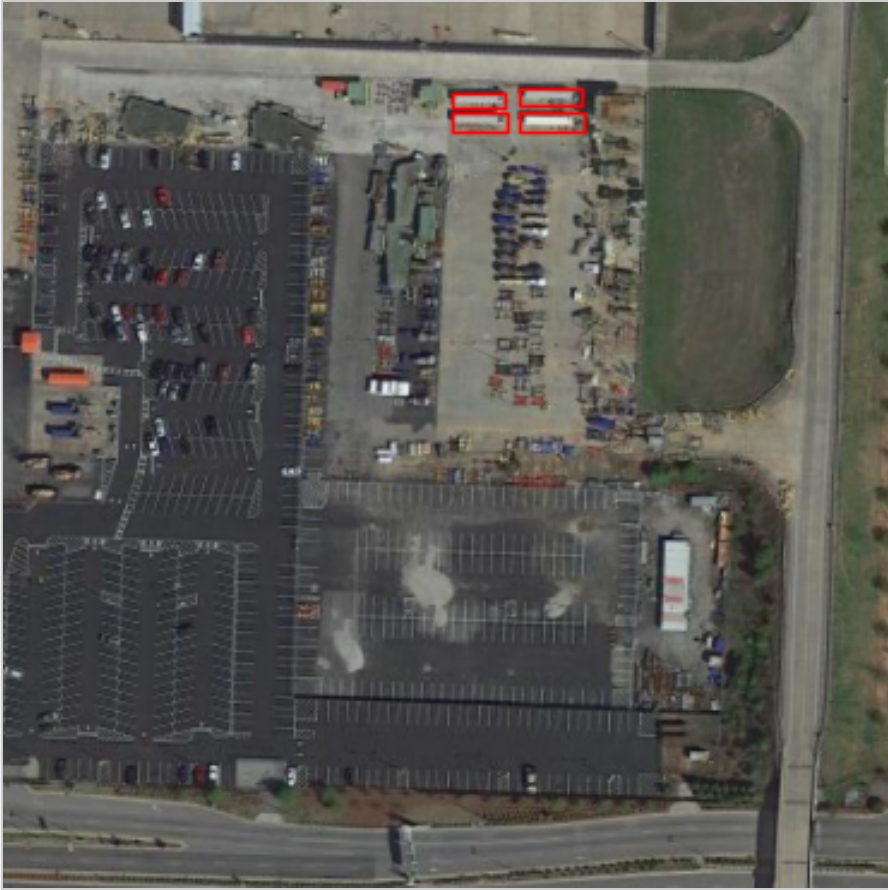
\includegraphics[width=0.7\textwidth]{./images/example_group.png}
\end{minipage}%
\begin{minipage}{0.5\textwidth}
\centering
\hspace{-1cm}
\raisebox{-0.3\height}{%
\footnotesize
\begin{tabular}{@{}p{2cm}p{5cm}@{}}
\toprule
\textbf{Expression Type} & \textbf{Example} \\
\midrule
Original & the group of 4 large vehicles in the top center \\
\midrule
Enhanced & the cluster of four big vehicles near the upper middle \\
\midrule
Unique & the four large vehicles lined up side by side just below the pale paved strip at the very top middle \\
\midrule
Unique & the set of four big vehicles parked in a single row in the upper center beside the grassy area to the right \\
\bottomrule
\end{tabular}%
}
\end{minipage}
\caption{Example of LLM enhancement process showing original aerial image with group of four large vehicles (left) and corresponding expression enhancements (right).}
\label{fig:llm_enhancement_example}
\end{figure*}


\begin{figure}[H]
\centering
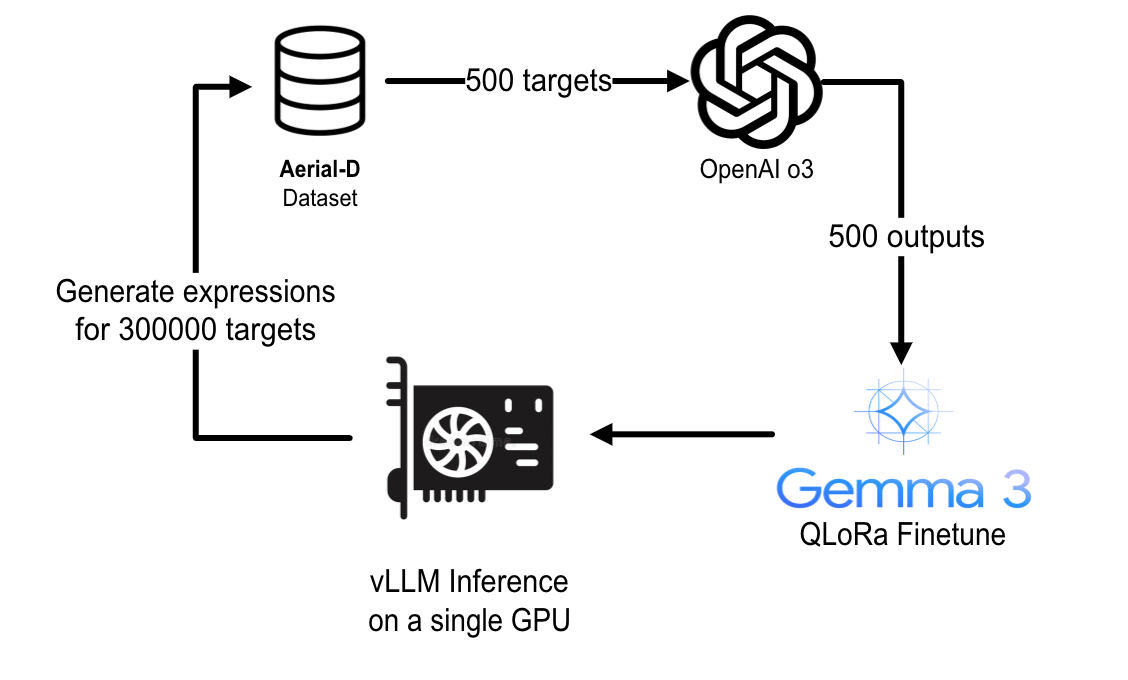
\includegraphics[width=0.8\columnwidth]{./images/distillation.png}
\caption{Knowledge distillation pipeline for scalable LLM enhancement. A small sample of 500 expressions is processed through OpenAI's O3 model to generate high-quality training targets, which are then used to fine-tune Gemma3 12B via QLora. The fine-tuned model enables cost-effective local inference to enhance the full dataset of 300,000 expressions using vLLM on a single GPU.}
\label{fig:llm_distillation}
\end{figure}

\subsection{Final Dataset Statistics}

The completed AerialD dataset represents a comprehensive resource for aerial referring expression segmentation, containing over 1.5 million expressions across diverse object categories and linguistic patterns. The dataset achieves substantial scale with 37,288 total patches containing 259,709 annotated samples, maintaining balanced distribution between individual objects (128,715 instances with 889,354 expressions) and groups (130,994 groups with 633,169 expressions).

The dataset encompasses both discrete objects from iSAID and semantic land cover categories from LoveDA, ensuring comprehensive representation of aerial imagery content. Small vehicles represent the most abundant category with 41,353 individual instances, while specialized categories like helicopters and baseball diamonds provide targeted coverage for specific aerial object types.

The systematic generation pipeline produces expressions through seventeen distinct templates, ranging from simple category references to complex multi-attribute descriptions. The LLM enhancement process successfully tripled the dataset size from 506,194 rule-based expressions to 1,522,523 total expressions, with nearly equal contributions from language variations (496,895) and unique visual detail expressions (519,434). This demonstrates the effectiveness of the two-pronged enhancement strategy in achieving both linguistic diversity and contextual richness essential for robust model training.

\begin{figure}[H]
\centering
\includegraphics[width=\columnwidth]{./images/expression_wordcloud.png}
\caption{Word cloud visualization of the most frequent terms in Aerial-D referring expressions, highlighting the domain-specific vocabulary and spatial descriptors characteristic of aerial imagery.}
\label{fig:expression_wordcloud}
\end{figure}

\begin{figure*}[t]
\centering
\begin{minipage}{0.48\textwidth}
\centering
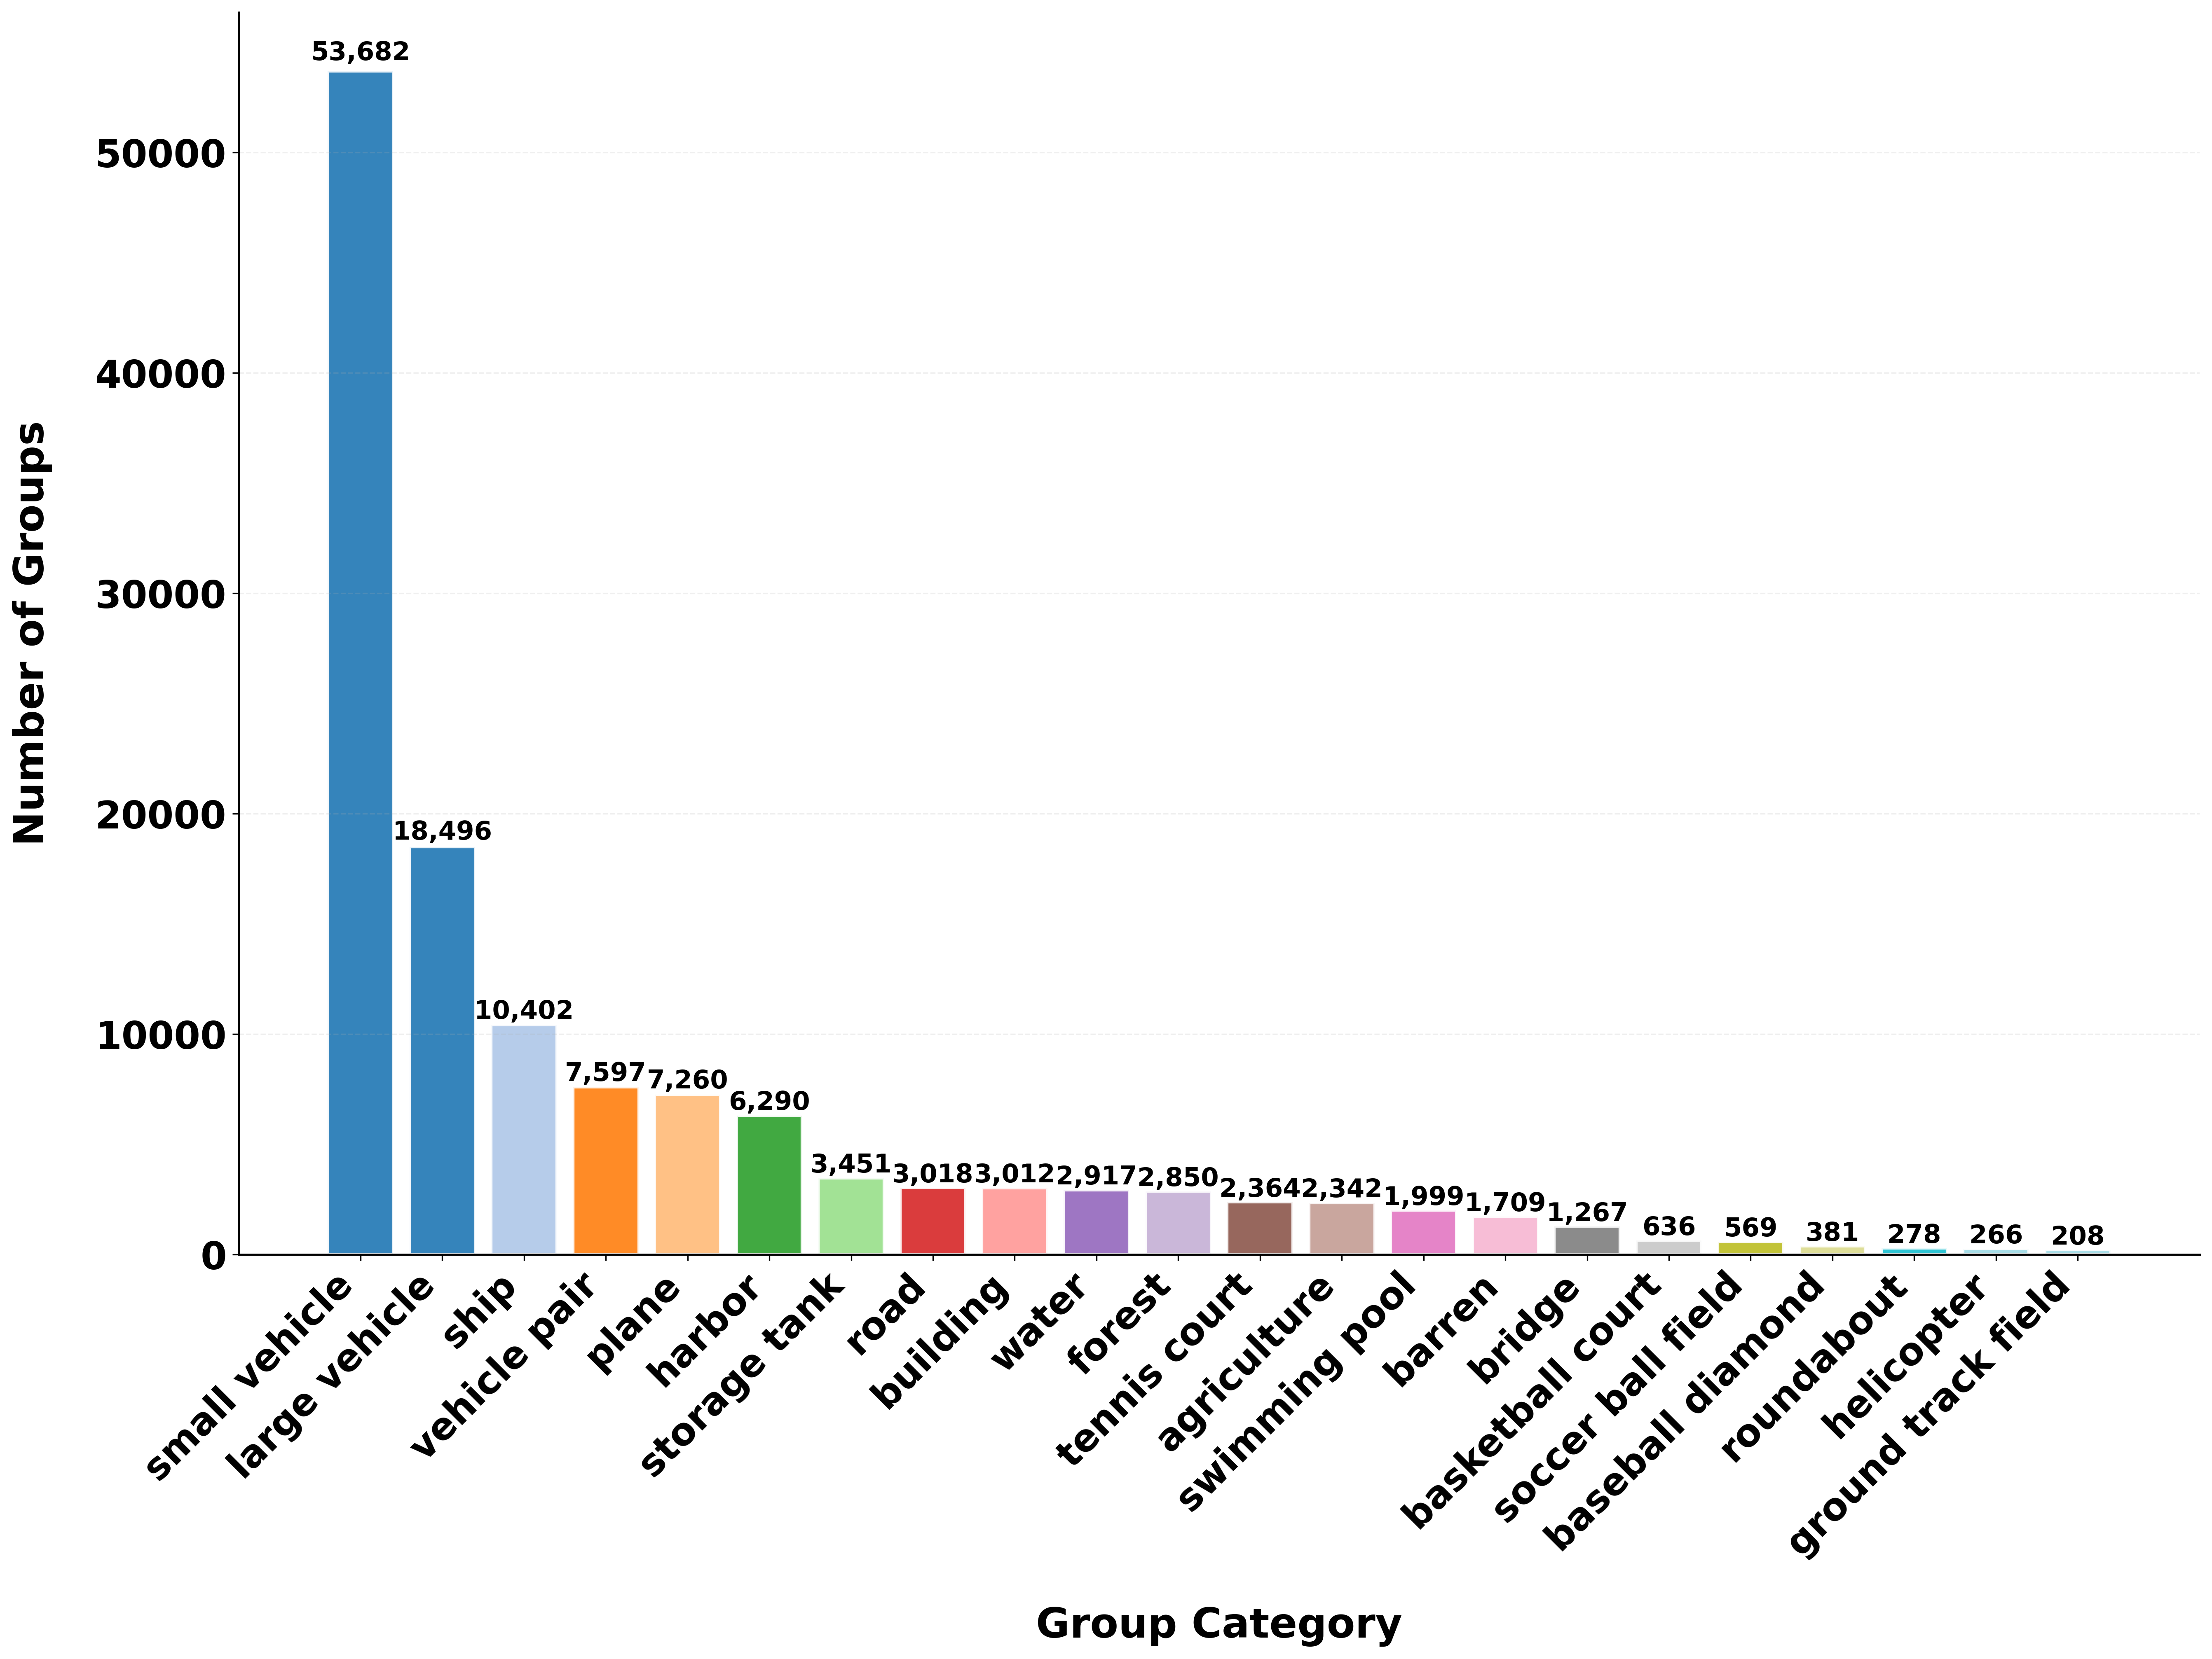
\includegraphics[width=\textwidth]{./images/group_category_distribution.png}
\end{minipage}\hfill
\begin{minipage}{0.48\textwidth}
\centering
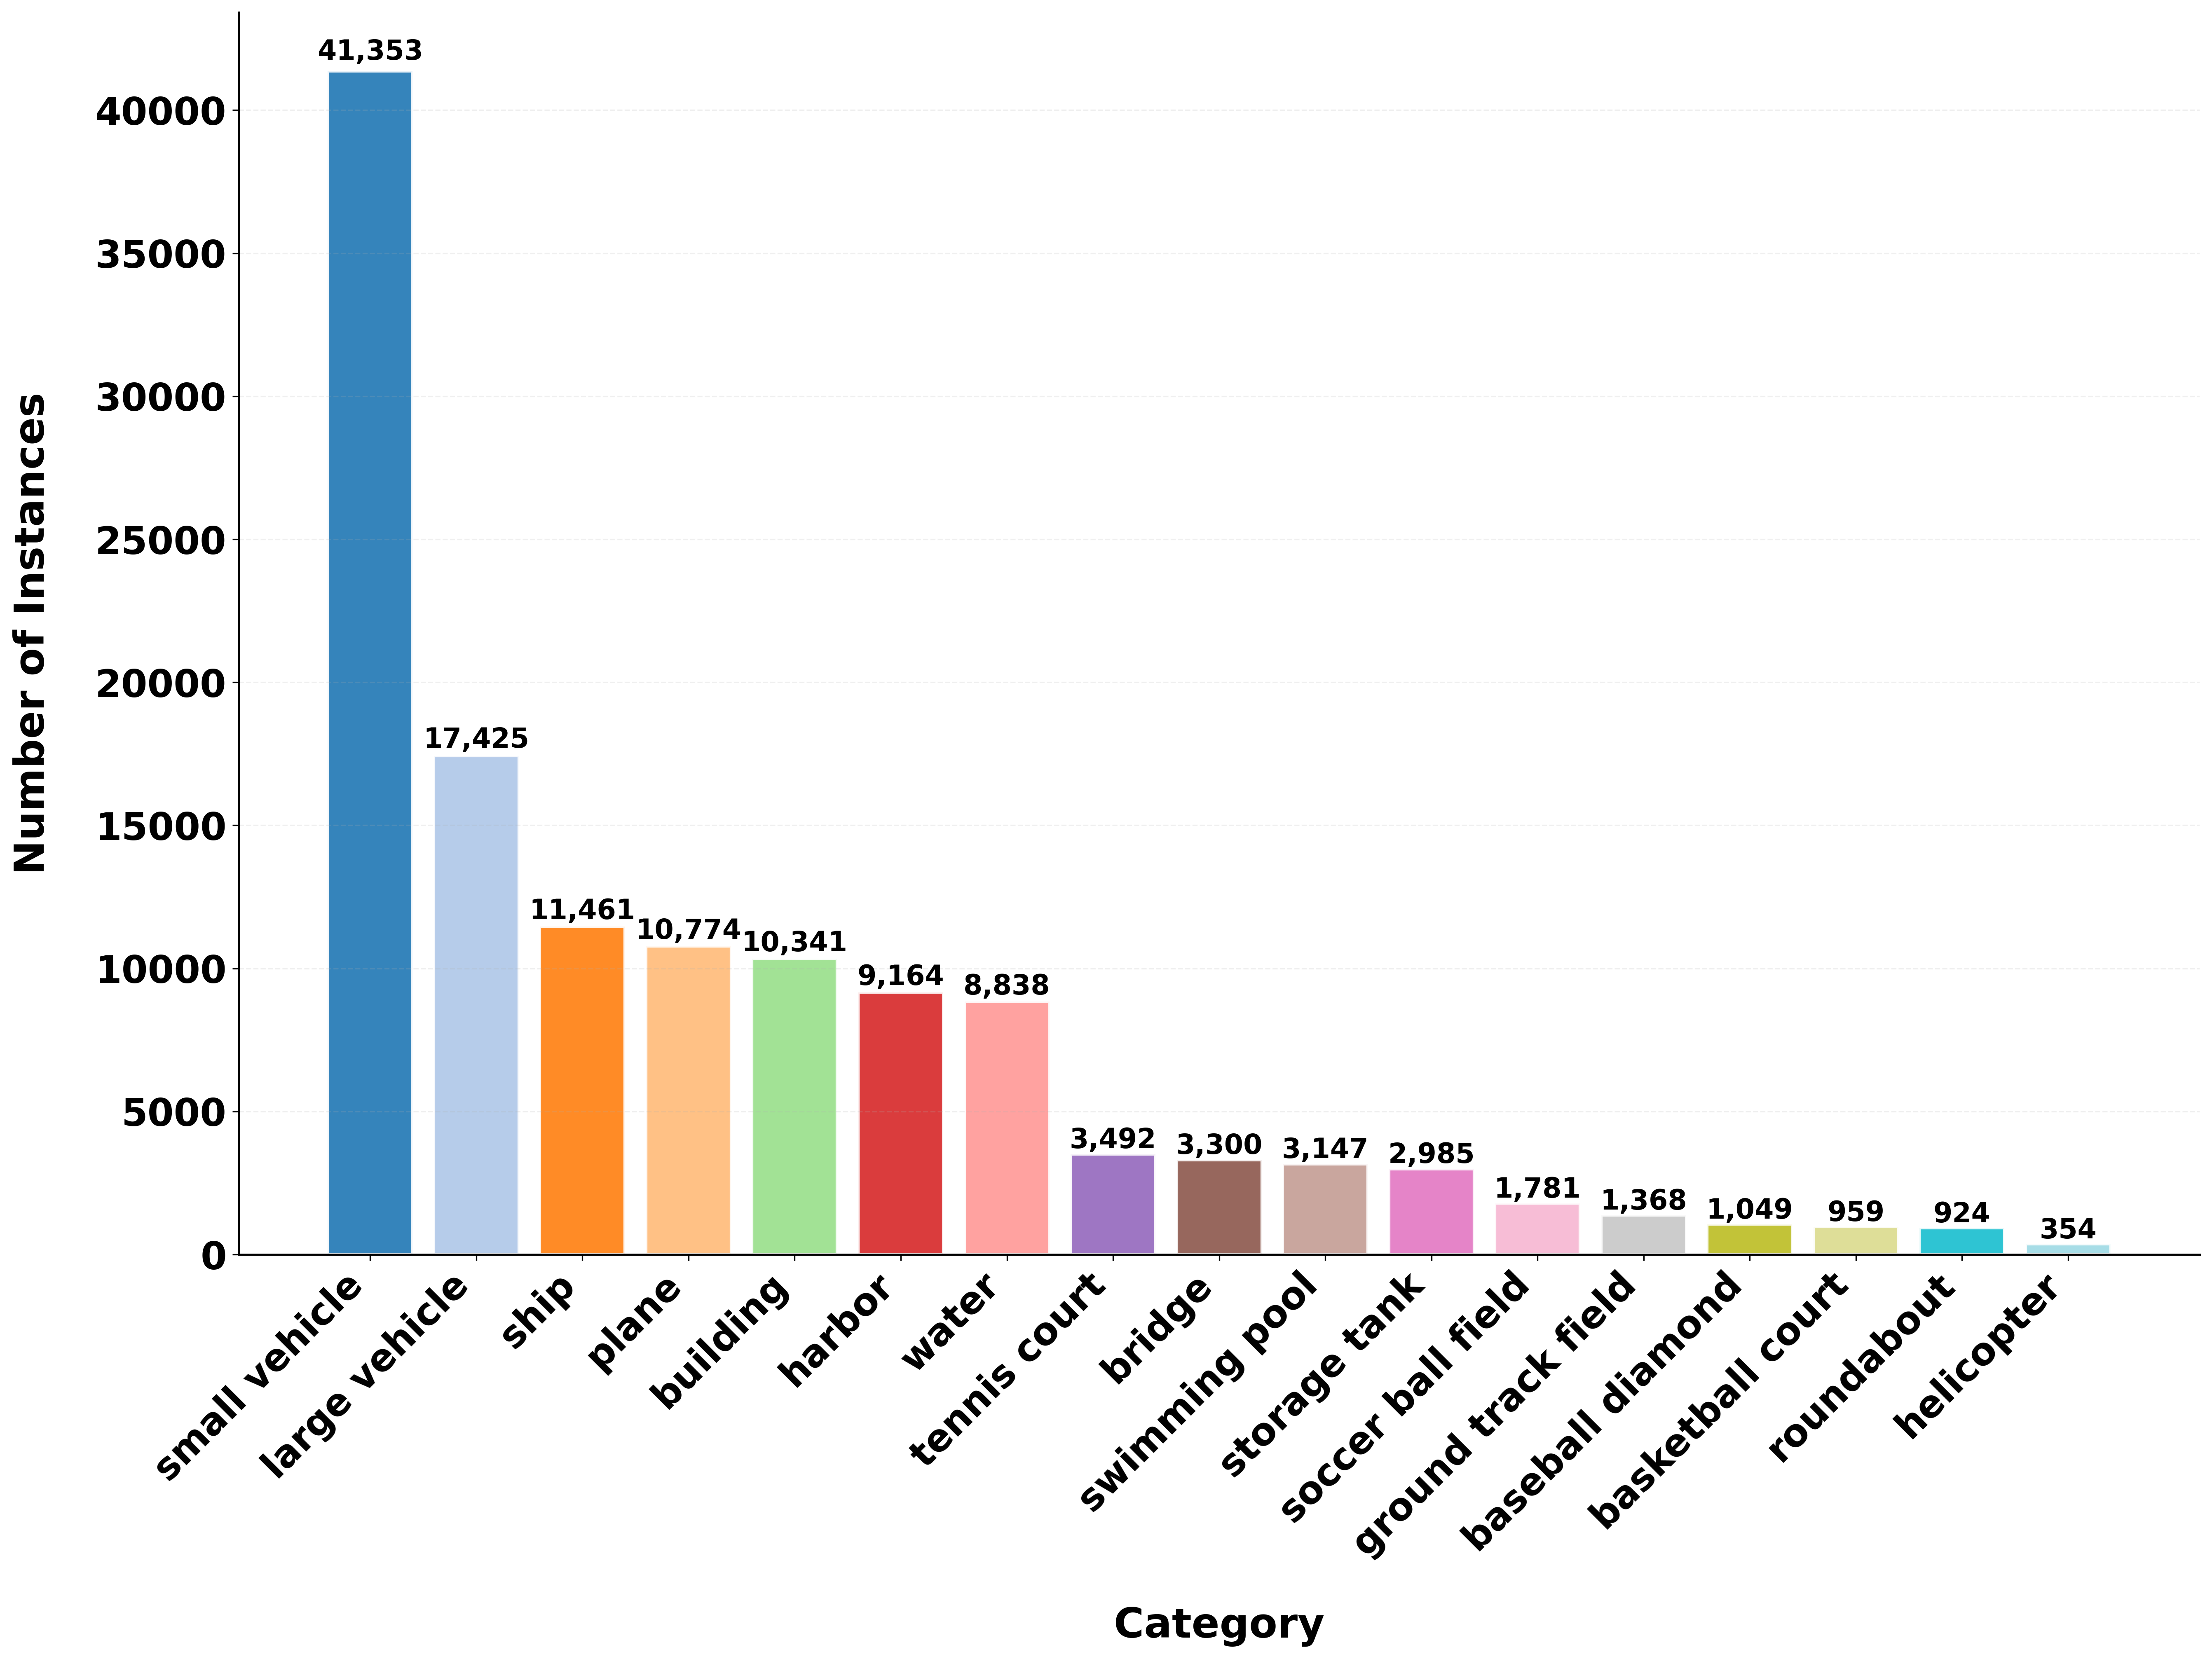
\includegraphics[width=\textwidth]{./images/instance_category_distribution.png}
\end{minipage}
\caption{Category distribution analysis of Aerial-D dataset. Left: Distribution of group annotations showing the prevalence of different object categories in group-level referring expressions. Right: Distribution of individual instance annotations across semantic categories, demonstrating the dataset's coverage of aerial object types.}
\label{fig:category_distributions}
\end{figure*}

Table \ref{tab:llm_enhancement_stats} quantifies the impact of LLM enhancement, showing that the distillation pipeline successfully tripled the dataset size from the original 506,194 rule-based expressions to 1,522,523 total expressions. The LLM enhancement process contributed nearly equal numbers of language variations (496,895) and unique visual detail expressions (519,434), demonstrating the effectiveness of the two-pronged enhancement strategy in achieving both linguistic diversity and contextual richness.

\begin{table}[H]
\centering
\caption{LLM Enhancement Expression Distribution}
\label{tab:llm_enhancement_stats}
\begin{tabular}{@{}lrrr@{}}
\toprule
\textbf{Expression Source} & \textbf{Train} & \textbf{Val} & \textbf{Total} \\
\midrule
Rule-Based Expressions & 371,360 & 134,834 & 506,194 \\
LLM Enhanced (Language Variations) & 364,396 & 132,499 & 496,895 \\
LLM Unique (Visual Details) & 382,038 & 137,396 & 519,434 \\
\midrule
\textbf{Total Expressions} & \textbf{1,117,794} & \textbf{404,729} & \textbf{1,522,523} \\
\bottomrule
\end{tabular}
\end{table}
